\documentclass[main.tex]{subfiles}

\begin{document}
\chapter{Phonon mediated tunneling into \TaS}\label{ch:sts_gap_tas2}

\section{Amplitude mode in \TaS charge density wave}\label{sec:amplitude_mode_tas2}

The results of the phonon calculation at the \(\mathrm{\Gamma}\) point carried out in sec. \ref{sec:phonon_tas2} are 81 phonon modes with respective energies and nucleic displacements.
One particular mode has the effect of displacing the atoms in the direction of the symmetric phase, thus changing the amplitude of the charge density wave.
This is depicted in fig. \ref{fig:amplitude_mode_tas2}.
The amplitude mode has an energy of \(E_0 = \SI{10.6}{\milli\eV}\).

\begin{figure}[b!]
    \centering
    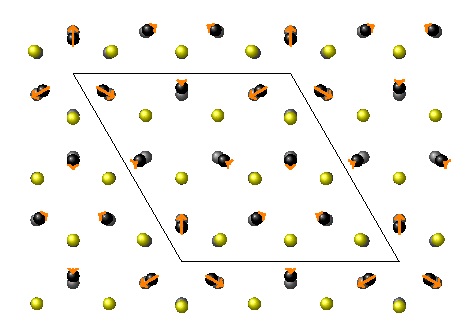
\includegraphics[width=0.5\textwidth]{higgs.pdf}
    \caption{Amplitude mode in \TaS charge density wave, visualized from \QE calculation. Gray dots are atoms in the symmetric phase, yellow/black dots are the Tantalum/Sulfur atoms in the charge-density-wave phase. The orange arrows show the displacement vectors.}
    \label{fig:amplitude_mode_tas2}
\end{figure}

\section{Phonon mediated tunneling into Graphene}

\subsection{Scanning Tunneling Spectroscopy}\label{sub:sts}

The description in this section follows the textbook \enquote{Surface Science} by Oura et al. \cite{oura_surface_2003}.

%\acrfull{sts} is an experimental technique in which a \acrfull{stm} is used to map the density of states of a material.

In an \acrshort{stm} setup, a ideally atomically sharp metallic tip is placed close to the probed surface (around \(\SIrange{5}{10}{\angstrom}\)), such that electrons can tunnel between the tip and the surface.
By applying a bias voltage \(V\) between the tip and the surface, a current enabled by the tunneling process flows through the gap.
This tunneling current is sharply dependent on the size of the gap, so a extremely high vertical resolution can be achieved.
Also due to this fact, \(\SI{90}{\percent}\) of the tunneling current flows through the the single tip atom closest to the surface, so that very high lateral resolution is also possible.
An \acrshort{stm} can thus be used to map the topography of a surface with atomic resolution.

When varying the bias voltage \(V\), an \acrshort{stm} can also be used to obtain measurements of the density of electronic states in the material, the \acrfull{sts} mode of operation.
This is due to the tunneling current being determined by summing over electron states in an energy interval defined by the bias voltage.
In general, a simple interpretation of \acrshort{sts} data is not possible and needs backing in theoretical calculations.
This is due to the tunneling current depending on the tunneling matrix element between the state at the tip and the states in the probe, so the tunneling current can be suppressed if the states in the probe don't overlap with the tip.

%Stipe et al. noted that the tunneling current in \acrshort{sts} can also identify phonon modes of the material measured \cite{stipe_single-molecule_1998} (vibrational modes of a single molecule in this case).

\subsection{Phonon mediated tunneling into Graphene}\label{sub:tunneling_graphene}

In a 2008 \acrshort{sts} measurement on graphene, a gap feature around the Fermi level was measured \cite{zhang_giant_2008}.
This gap is an example of the problems with interpretation of \acrshort{sts} data explained in sec. \ref{sub:sts}, as it is not a feature of the density of states of graphene, but a result of the tunneling current being suppressed for the range of bias voltages in the gap.

The underlying mechanism, confirmed with \acrshort{dft} calculations by Wehling et al. \cite{wehling_phonon-mediated_2008} is as follows:
generally, electrons can elastically tunnel into graphene at the Fermi level near the \(\boldsymbol{K}\) point.
This elastic process is suppressed because the wave function at the initial state, i.e. the wave functions at the tip, have a momentum distribution centered at \(\vb*{k}_{\parallel} = 0\), so the tunneling matrix element is suppressed for large \(\vb*{k}\) \cite{vitali_phonon_2004}.
For electron energies outside the gap, an inelastic tunneling channel opens, where the electrons first tunnels into the \(\sigma^*\) band and then transitions into an available \(\boldsymbol{K}\) point through emission of a \(\boldsymbol{K}^{\prime}\) point phonon (pictured in fig. \ref{fig:graphene_tunneling}).

\begin{figure}
    \centering
    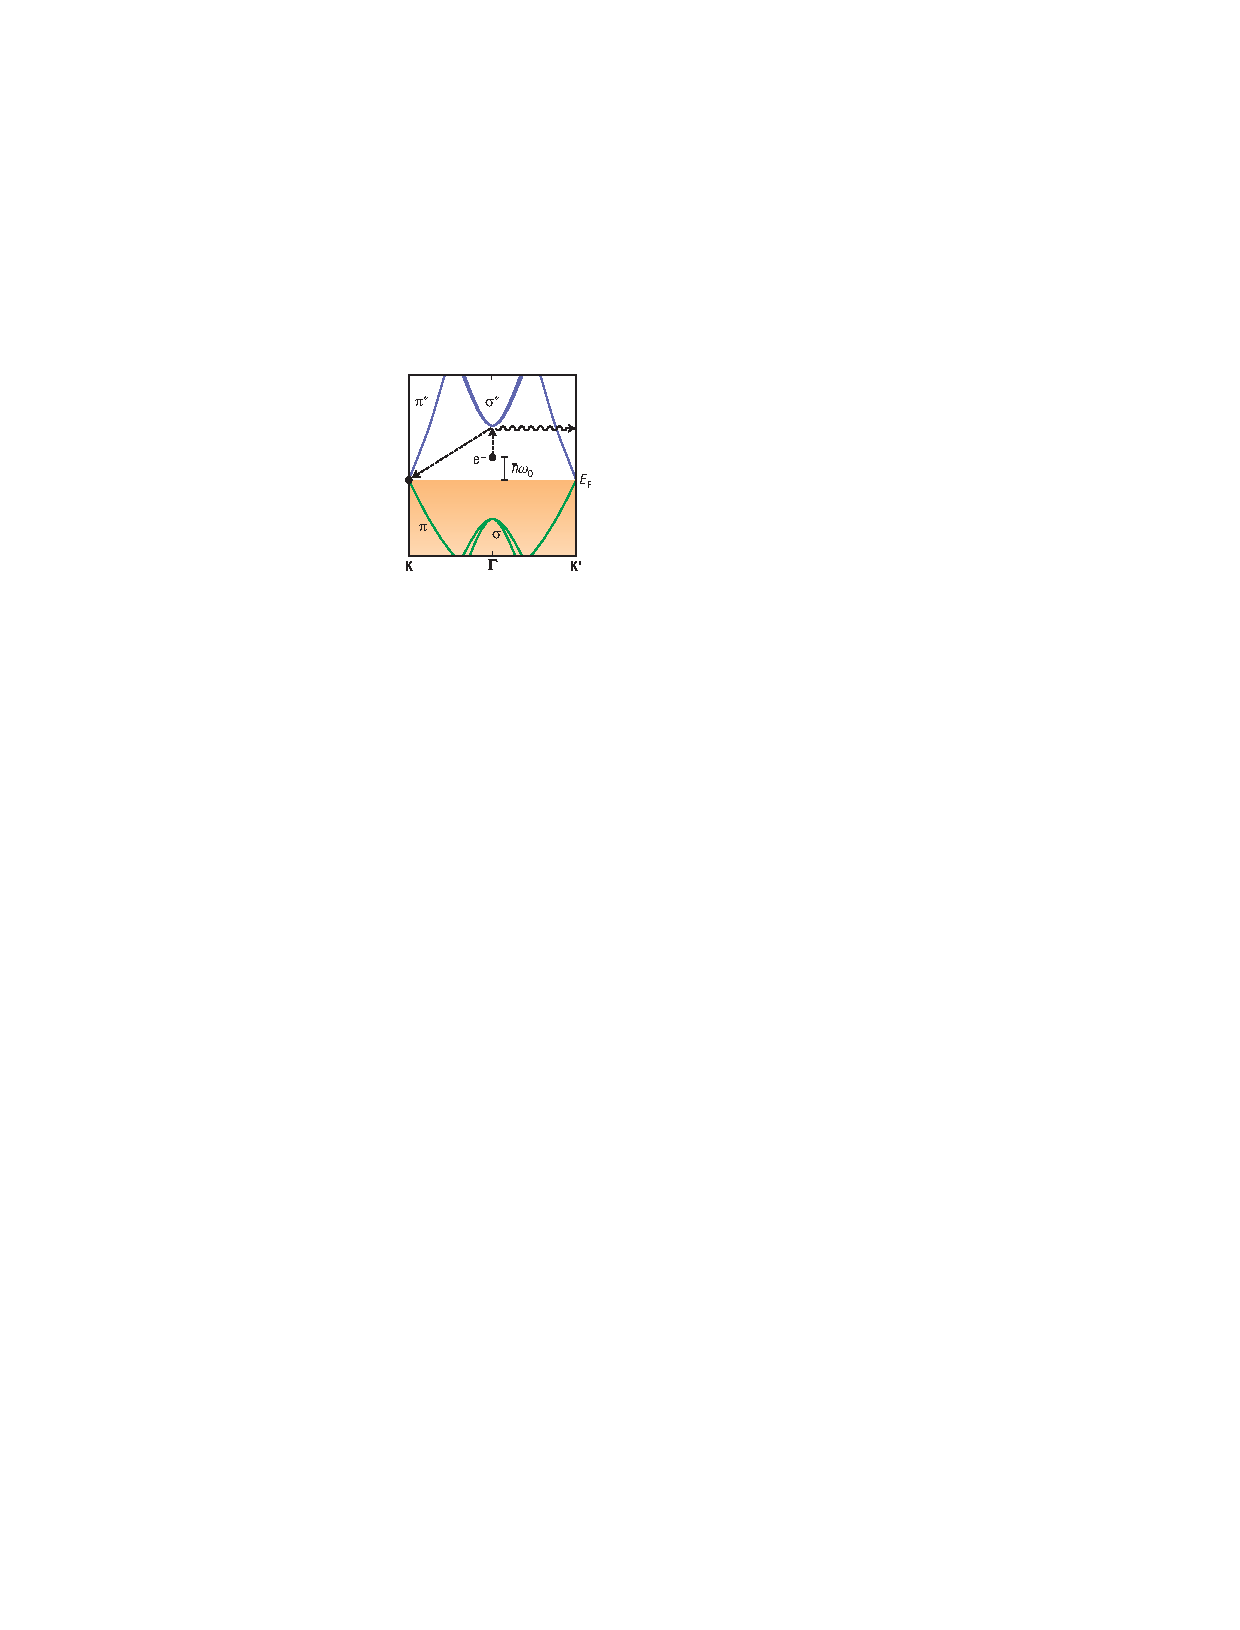
\includegraphics[width=0.3\textwidth]{graphene tunneling.pdf}
    \caption{Inelastic tunneling mechanism involving graphene phonon modes near the \(\boldsymbol{K}\) point in reciprocal space. \emph{Reprinted by permission from Nature Publishing Group: Nature Physics \cite{zhang_giant_2008}, \copyright\, 2008}}
    \label{fig:graphene_tunneling}
\end{figure}

%\clearpage
\section{Phonon mediated tunneling into \TaS}

In a 2019 paper by Hall et al. \cite{hall_environmental_2019}, a similar gap feature with a width of \(2 \Delta = \SI[separate-uncertainty = true]{32 \pm 9}{\milli\eV}\) was reported in an \acrshort{sts} measurement on \TaS.

This gap is attributed to partial gapping to the formation of the charge density wave, as explained in the one-dimensional case in sec. \ref{sec:systems_tas2}.

\begin{figure}
    \centering
    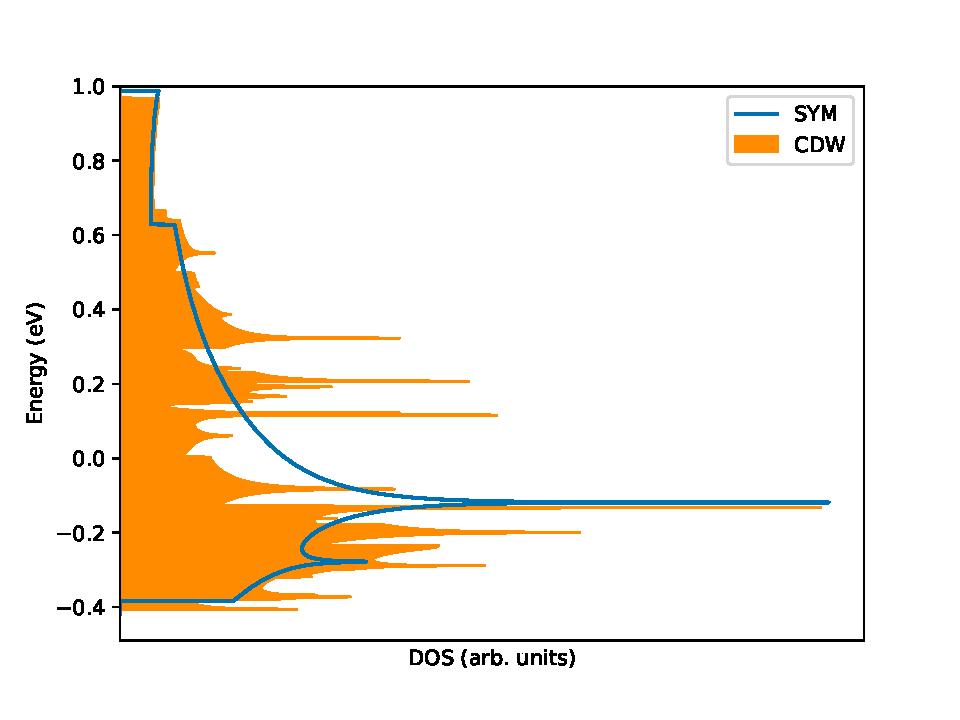
\includegraphics[width=0.6\textwidth]{tas2_dos.pdf}
    \caption{Density of states for \TaS in the charge density wave (CDW) and undistorted (SYM) phase. The data was kindly provided by Dr.\,Jan Berges and has been calculated in \QE with the 2D tetrahedron method using 360² (1080²) \(k\) points for the CDW (SYM) structure}
    \label{fig:tas2_dos}
\end{figure}
The density of states depicted in fig. \ref{fig:tas2_dos} shows no symmetric gap around the Fermi level, hence the explanation by partial gapping is not confirmed.
An alternative explanation can be that the same process found in graphene in sec. \ref{sub:tunneling_graphene} produces the gap in \TaS.
The gap \(\Delta = \SI[separate-uncertainty = true]{16 \pm 4.5}{\milli\eV}\) could be explained with an inelastic tunneling process involving the amplitude mode near the \(\Gamma\) point with an energy around the calculated \(E_0 = \SI{10.6}{\milli\eV}\).
Confirmation of this explanation would need an ab initio model of the electron-phonon interaction and its effects on the tunneling, similarly to graphene \cite{wehling_phonon-mediated_2008}.

\end{document}